\documentclass[conference]{IEEEtran}

\usepackage[english]{babel} 
\usepackage[utf8]{inputenc}
\usepackage[T1]{fontenc}
\usepackage{cite}
\usepackage{url}
\usepackage{hyphenat} % For linebreaks
\usepackage{hyperref}
\usepackage{geometry}
\usepackage{graphicx} % IncludeGraphis
\usepackage{caption} % Subfigure
\usepackage{subcaption} % Subfigure

% correct bad hyphenation here
% \hyphenation{op-tical net-works semi-conduc-tor}


\begin{document}

\title{Stream processing with Twitter Heron}

\author{\IEEEauthorblockN{Adrian Bartnik}
\IEEEauthorblockA{Technische Universität Berlin\\
Email: bartnik@campus.tu-berlin.de}}

\maketitle

\begin{abstract}
This paper gives an overview about the requirements and the demands of a real-time stream processing platform.
As an example, it presents the architecture and design decisions of Apache Storm, its successor Twitter Heron and Google`s MillWheel. % Asumptions?
It compares each streaming platform in terms of prior assumptions, scalability and extensibility.
Finally, it presents a summary with the advantages and disadvantages of each platform and gives an outlook for future use cases.

\end{abstract}

\section{Introduction}
\label{sec:Introduction}

In recent years, stream processing has become a new companion to the family of big data buzzwords.
It describes the paradigm of processing incoming high-volume data stream, where the data can come from various sources.
Scenarios are micro transactions at a stock exchange, sensor measurements from small independent devices in the upcoming area of the Internet of Things or analytic data coming in from millions of mobile phones.

Most major Internet-scale companies either have their own proprietary stream processing platform or use some open-source alternative.
One prominent example is Twitter, a real-time messaging service with over 320 million active users and over 1 billion unique site visits each month.
Twitter uses stream processing in various places, for example to compute the trending topics, a small section on their website showing the currently most used, and therefore most relevant keywords by their users.
In 2011 Twitter started off developing its own stream processing platform Twitter Storm after acquiring the technology from the company BackType.
Shortly afterwards, they also made the whole project available under open source and it became an Apache top-level project.

But, using Storm at its scale was becoming increasingly challenging due to issues related to scalability, debug-ability, manageability, and efficient sharing of cluster resources with other data services.
The company therefore started to develop a new system, Twitter Heron, which should fix their problems and also be able to scale for the future.
Twitter Heron is now the de facto stream data processing platform inside Twitter.

The rest of the paper is organized as follows: The following section, Section \ref{sec:Background}, describes the characteristics of real-time stream processing and the requirements of a stream processing platform.
Section \ref{sec:RelatedWork} describes other platforms and related work.
Section \ref{sec:ApacheStorm} and \ref{sec:TwitterHeron} describe Apache Strom and Titter Heron respectively, where the later also describes the evolution between the two platform.
The evaluation in section \ref{sec:Evaluation} compares both approaches.
Finally, section \ref{sec:Conclusion} contains the conclusion.

\section{Background}
\label{sec:Background}

This section explains the fundamentals of stream processing and the characteristics and requirements of a stream processing platform respectively.

\subsection{Real-time Stream Processing}
\label{sec:RealTimeStreamProcessing}

The major distinction between plain big data and stream processing is, that the later operates on \emph{unbounded data}.
This means, that the size of the input is ever-growing and essentially infinite, whereas usually the input size is typically limited by either the file or database size and known in advance \cite{WorldBeyondBatch}.

Generally speaking, stream processing describes a one-at-a-time processing model, where each data item is arriving separately and is independent from the rest.
This holds true for most use cases, such as financial transactions, sensor measurements from different devices or in Twitter's case \emph{tweets}.
As results should be available as fast as possible, the items should be process upon arrival and not be combined into batches.
The goal is typically to achieve sub-second latency \cite{BeyondBatchProcessing}.

The computations of a stream processing platform on the incoming data should ideally be simple, independent and separated.
This way it becomes easier to distribute the computations onto different machines in one cluster and thus the whole platform can scale better.
In many systems the computations on the data form a directed acyclic graph, e.g. the jobgraph in Flink or, as we will see, a topology in Heron \cite{Flink}.
Finally, all computations should happen in-memory, because writing intermediate results to disk would introduce a big delay compared to pure memory access.

% TODO Exactly, at most/least once processing

\subsection{Requirements of a Stream Processing Platform}
\label{sec:RequirementsOfAStreamProcessingPlatform}

In 2005, Michael Stonebraker et al. outlined eight requirements that a system should meet to excel at a variety of real-time stream processing applications.
They provide high-level guidance when evaluating alternative solutions \cite{The8Requirements}.
Later on, these requirements will be compared to Apache Storm and Twitter Heron.

\begin{LaTeXdescription}
  \item[1) Keep the data moving] The data should be processed \emph{in-stream}, without a requirement to be stored on disk to perform additional operations
  \item[2) Query using SQL on Streams] Support a high-level “StreamSQL” language with built-in extensible stream-oriented primitives and operators.
  \item[3) Handle Stream Imperfections] Provide resiliency against stream “imperfections”, including delayed, missing and out-of-order data.
  \item[4) Generate Predictable Outcomes] A stream processing platform must guarantee predictable and repeatable outcomes.
  \item[5) Integrate Stored and Streaming Data] The system should be able to integrate live and stored data seamlessly and to have the capability to efficiently store, access and modify state information.
  \item[6) Guarantee Data Safety and Availability] Ensure that the system is up and available, and the integrity of the data maintained at all times, despite failures.
  \item[7) Partition and Scale Applications Automatically] The system should enable incremental scalability across multiple processors or machines, ideally automatically and transparent.
  \item[8) Process and Respond Instantaneously] The stream processing system must have a highly-optimized, minimal-overhead execution engine to deliver real-time response for high-volume applications.
\end{LaTeXdescription}

\begin{figure*}[!h]
\centering
	\begin{subfigure}{1.35\columnwidth}
		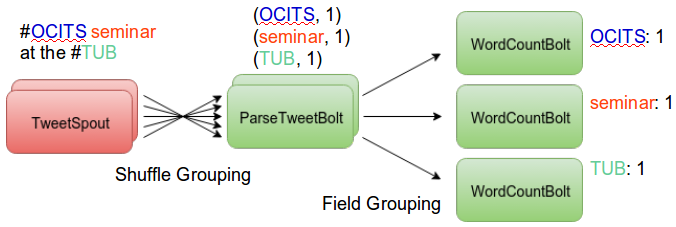
\includegraphics[width=\columnwidth]{figures/TopologyWordCount}
		\caption{The trending topics topology}
		\label{fig:TopologyTrendingTopics}
	\end{subfigure}\hspace{2.9em}
	\begin{subfigure}{.55\columnwidth}
		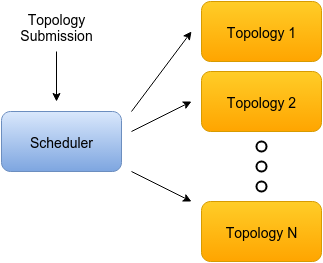
\includegraphics[width=\columnwidth]{figures/TopologySubmission}
		\caption{The overview of the \\topology submission}
		\label{fig:TopologySubmission}
	\end{subfigure}\hfill
\label{TopologyDescription}
\caption{Overview of topologies in Apache Storm and Twitter Heron}
\end{figure*}

\section{Related Work}
\label{sec:RelatedWork}

It might seem, that processing high volume data streams has just become a big research area in recent years by internet-scale companies, but the most systems build on top of work done from over a decade ago (\cite{StreamStanford, Aurora}).
In 2013, Google published their solution called MillWheel \cite{Millwheel}, which is not a complete system such as Apache Storm, but a "framework for building low-latency data-processing applications".
The paper states, that it is currently widely used at Google, but the source code is not available.
With Milwheel, Google focuses particularly on low latencies and exactly-once processing, which is neither available in Storm nor Heron.
Finally, they say that their framework fulfills all eight requirements for a streaming system by Stonebraker et al., which were described previously.

Two open-source alternatives are Spark Streaming, which focuses on parallel recovery mechanisms and consistency across multiple nodes.
They claim, their system scales linearly up to 100 nodes and at the same time provide subsecond latency and fault recovery \cite{SparkStreaming}.
And lastly, also Apache Flink, which started at the TU Berlin, and recently seems to be gaining commercial traction \cite{FlinkUpcoming}.
Its biggest advantage is, that is supports batch and stream processing alike \cite{Flink}.

\section{Apache Storm}
\label{sec:ApacheStorm}

Storm was Twitter's real-time distributed stream data processing engine, that powered the data management tasks and was crucial to provide Twitter services.
During the design of Storm, they wanted the system to be scalable, so that is easy to add or remove nodes from the cluster without disrupting running tasks.
It should be resilient as hardware component failures are the rule rather than the exception, and the cluster should continue processing existing topologies with a minimal performance impact.
Furthermore, the system should be extensible, because future requirements are not known in advance, e.g. what services or components will be added the whole infrastructure, and it should adjust accordingly.
Storm must also be highly performant, as it powers real-time applications and Twitter is running at a huge scale with millions of users.
Last but not least, the whole system must be easy to administer, because it plays a big part in the user interaction and issues (performance or failure) will be therefore be immediately noticed.
Thus, Storm needs to provide easy-to-use administrative tools and should emit warnings as soon as possible.

\subsection{Data model}

The heart of Strom's data model is a \emph{topology}, a directed acyclic graph of nodes as shown in figure \ref{fig:TopologyTrendingTopics}.
It represents a logical view on how the data is flowing though the system.
A \emph{spout}, the red node, is responsible for managing and piping incoming data into the topology, where the data can come from various sources: live data, message brokers (e.g. Kafka)  or a database.
The counterpart is a \emph{bolt}, which is an abstraction for any kind of processing or computation, that we want to execute on the data items.
In a topology, every spout or bolt is shown as a single node, but in a real cluster execution, the programmer has to manually specify how many instances of a spout or bolt are spawned.
The data flow between the spout and bolt instances is defined by different partition strategies, e.g. \emph{Global grouping}, which sends the entire stream to a single bolt.
To sum it up, a topology is a directed acyclic graph of spouts and bolts, that represents the logical flow of data through Storm \cite{StormTwitter}.

One example of a real-world topology is shown in figure \ref{fig:TopologyTrendingTopics}, which display the trending topics section on Twitter's homepage.
It counts the currently most used words by the users and computes the 10 most relevant words.
Here, the incoming tweets are received at the TweetSpout, which forwards the message content to some random ParseTweetBolt instance via the \emph{Shuffle Grouping} partition strategy.
This bolt parses the message, filters common words and creates tuples with the word and the number of occurrences.
It then forwards this tuple based on the word using the \emph{Field Grouping}, where one instance of the WordCountBolt receives all the tuples with the same key.
And finally every 5 minutes, these bolt instances output their current state and a new version of the trending topics sections gets computed.

\subsection{Architecture}

\begin{figure*}[!h]
\centering
	\begin{subfigure}{.55\columnwidth}
		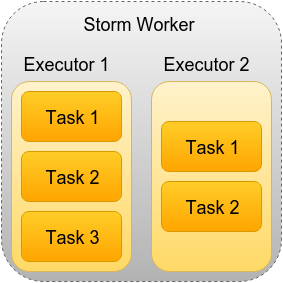
\includegraphics[scale=0.35]{figures/StormWorker}
		    \caption{The overview of the Storm Worker}
		    \label{fig:StormWorkerOverview}
	\end{subfigure}\hspace{2.9em}
	\begin{subfigure}{1.35\columnwidth}
		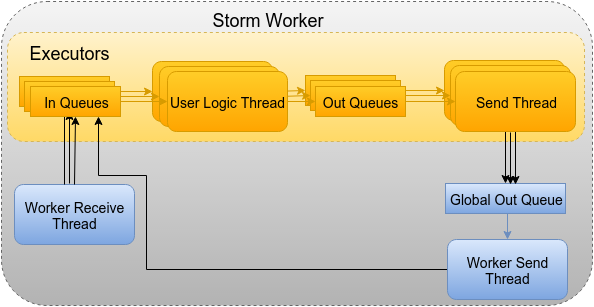
\includegraphics[scale=0.35]{figures/StormWorkerDetail}
		    \caption{The internals of the Storm Worker}
		    \label{fig:StormWorkerDetail}
	\end{subfigure}\hfill
\label{fig:StormArchitectureOverview}
\caption{Overview of Apache Storm architecture}
\end{figure*}

Clients submit topologies to a master node, which called the \emph{Nimbus} and handles the scheduling of all topologies (Figure \ref{fig:TopologySubmission}).
The Nimbus is responsible for distributing, coordinating and monitoring the execution of the topology.
A more detailed view of the architecture of Storm is shown in figure \ref{fig:StormArchitecture}.
The state and status of the cluster is maintained by ZooKeeper \cite{Zookeeper}.
The actual work is done in the \emph{Worker Nodes}, which each host a \emph{Supervisor} and multiple \emph{Storm Worker}.
The supervisor is responsible for communicating with the Nimbus via a periodic heartbeat protocol to advertise the execution state or to inform him about free resources to run more work.
He also starts or stops Storm Workers, which are the units, that get scheduled by the Nimbus \ref{fig:StormArchitecture}.

\begin{figure}[!hb]
		\includegraphics[width=\columnwidth]{figures/StormArchitecture}
		\caption{The overview of the \\topology submission}
		\label{fig:StormArchitecture}
\end{figure}

The general and also the detail architecture of a Storm Worker are shown in figures \ref{fig:StormWorkerOverview} and \ref{fig:StormWorkerDetail}.
Each Storm Worker runs as one single JVM process and contains multiple \emph{Executors}, which in turn contain multiple tasks.
One Storm Worker always belongs to one topology, but multiple Workers on the same machine may be executing different parts of the same topology.
Each task is one instance of either a bolt or a spout and does actual work on the incoming data.
Executors are just threads inside a Storm Worker and bundle multiple tasks.
Thus, tasks provide intra-bolt/intra-spout parallelism, and the Executors provide intra-topology parallelism.
Storm Worker serve as containers on the host machines to run Storm topologies.

The detail architecture of a Storm Worker is shown in figure \ref{fig:StormWorkerDetail}.
The routing of incoming and outgoing tuples inside a Worker is implemented via two global threads, the \emph{Worker Receive Thread} and the \emph{Worker Send Thread}, which handle the reception and sending respectively.
An Executor consists of the 2 Threads.
The \emph{User Logic Thread} takes incoming data from the \emph{In Queue}, executes the corresponding tasks (spout or bolt instances) and writes the result to the \emph{Out Queue}.
For outgoing tuples that are destined for a different task on the same worker, the Executors \emph{Send Thread} writes the tuple directly into the In Queue of the destination task.
Otherwise, it will send the tuple to the \emph{Global Out Queue}.

\begin{figure*}
	\centering
    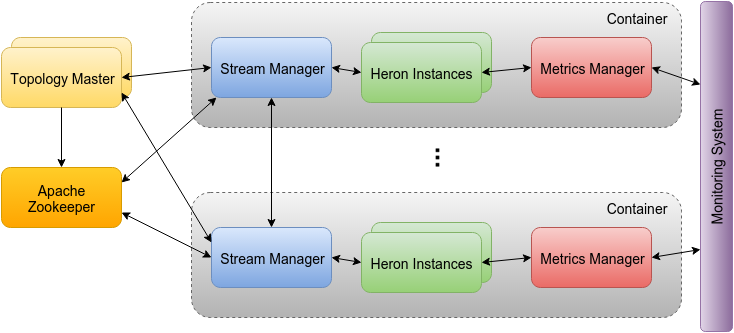
\includegraphics[scale=0.35]{figures/HeronOverview}
    \caption{The overview of Heron}
    \label{fig:HeronOverview}
\end{figure*}

\section{Twitter Heron}
\label{sec:TwitterHeron}

Using Storm in production for several years, Twitter experienced that the system does not fulfill some desired properties: scalability, debuggability and performance.
In Storm, work from multiple components of a topology is bundled into one operating system process, which makes debugging very challenging.
When a topology misbehaves – which could be for a variety of reasons including load changes, misbehaving user code, or failing hardware – it was hard to determine the root-cause for those problems.
Thus, a cleaner mapping from the logical units of computation to each physical process was needed \cite{TwitterHeronBlog, TwitterHeron}.

In addition, Storm needed dedicated cluster resources, which required special hardware allocation to run Storm topologies.
This approach leaded to inefficiencies in using precious cluster resources, and also limited the ability to scale on demand.
A more flexible way in scheduling popular cluster resources across different types of data processing system (not only stream processing) was needed.

Moreover, Storm did not provide an automated way of provisioning new or decommissioning old topologies, which required a lot of manual cluster management.
The new system should be easier to manage, which would lead to a more efficient system and thus, at Twitter's scale, reduce infrastructure costs and also significantly improve the productivity of the cluster management.

\subsection{Evolution from Apache Storm}
\label{sec:EvolutionFromApacheStorm}

The major reason not to use an existing open-source alternative for their new system was driven by the fact, that Twitter was heavily dependent on existing Storm topologies for their production system.
Instead, they decided to design a new system, Heron, for which the compatibility with the Storm and Summingbird API was essential.
Summingbird provides a Scala-idiomatic way for programmers to express their computation and constraints generates many of the Storm topologies that are run in production \cite{Summingbird}.
By maintaining the old API, Twitter could simple reuse all existing topologies, as well as all adjacent systems in their ecosystem, and the way one interacts with the programming model in terms of spouts, bolts and topologies remained the same.

\begin{figure*}
    \centering
    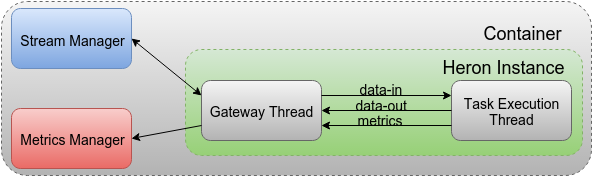
\includegraphics[scale=0.35]{figures/HeronInstance}
    \caption{The internals of a Heron Instance}
    \label{fig:HeronInstance}
\end{figure*}

\subsection{Architecture}
\label{sec:TwitterHeronArchitecture}

Heron also relies on Apache Zookeeper for the cluster management, but additionally implements an abstraction layer for various other scheduler (YARN, Mesos and ECS \cite{Aurora, YARM}, that makes it easy to run topologies on other clusters.
The \emph{topology master} is responsible for maintaining the lifecycle of the topology, which can be supported by a standby topology master for availability.
This is a huge improvement compared to Storm, where the Nimbus was a single point of failure.
Figure \ref{fig:HeronOverview} gives an overview of Heron's architecture.

The equivalent of a Storm Worker is call simply container, which hosts a \emph{Stream Manager}, a \emph{Metrics Manager} and several \emph{Heron Instances}.
Each Heron Instance connects to its local SM to send and receive tuples.
The Stream Manager's task is to manage the tuple routing efficiently, so it either sends the tuples to Heron Instances in the same container locally or to a Stream Manager in another container.
The Metrics Manager of each container collects and exports metrics from all the components in the system, e.g. about the system or topology status, and send them to the monitoring system.
Compared to Storm, the biggest change is the Heron Instance, which is the realization either a tweet or a spout.
Since the complexity of data movement has been moved to the Stream Managers, native Heron Instances in different languages could be supported in the future.

A Heron instance, shown in figure \ref{fig:HeronInstance}, consists of 2 threads, the \emph{Gateway} and \emph{Execution Thread}, and 3 queues for communicating between each other.
The queues are bound in size and if they reach their limit, a backpressure mechanism informs the Stream Manager to slow down the sending of tuples.
The whole instances is implemented in a single JVM making it easier to predict the resource consumption and also improves debuggability to identify failures.

\section{Evaluation}
\label{sec:Evaluation}

Comparing Storm and Heron to Stonebraker's paper in section \ref{sec:RequirementsOfAStreamProcessingPlatform}, we see that Heron fulfills all 8 whereas Storm only fulfills 7 requirements.
Both systems provide a framework for using high-level stream-oriented operators, Summingbird, required by point 2.
Through the input abstractions via spout, they make it easy to pull data in from various sources into a topology, described by point 5.
Although both systems provide scaling mechanism, Heron is superior in the way how efficient and performant it is able to do so.
The Nimbus, the single point of failure in Storm, is the reason why this system does not meet point 6: availability.

Comparing both system, we encounter various problems with the design of the Storm Worker.
Starting off, it introduces scheduling decision on multiple levels: First, the underlying machine has to choose one Storm Worker to execute, which then contains multiple Executors with User Logic and Send Threads.
Finally, the former may has to select between multiple tasks to run.
In addition, an Executor may run disparate tasks, which makes it really hard to reason about the runtime behavior and especially the resource consumption.
Furthermore, because each Storm Workers runs as a single JVM, debugging in case of failure becomes a nightmare.
And lastly, the whole design introduces a lot of overhead, as each tuple has to pass 4 threads before being completely processed.

Heron solves these problems, while maintaining consistency with the old API.
The biggest improvement is the clean separation between routing logic and tuple processing trough the Stream Manager and Heron Instance.
Combined with the fact, that each Heron Instance is using its own JVM and is running one specific task, this leads to a more fine grained predictability about runtime behavior, resource consumption and debuggability.
Having a direct link between Heron Instance and Stream Manager also enables the system to implement backpressure mechanisms for controlling the volume of incoming tuples.
The major performance advantage comes from the fact, that a Heron Instance uses fewer threads and queues for tuple processing and outsources monitoring to a separate component of the system.
And last but not least, Heron does not have a single point of failure anymore.  

\section{Conclusion}
\label{sec:Conclusion}

We have seen, that processing high-volume data streams has many use-cases in the real-word: from financial transaction over sensor measurements up to Twitter's messaging service.
The main characteristics are an unbounded input data size with a one-at-a-time processing model, where the computations should be kept simple and independent and ideally happen upon arrival and "in-stream".

We looked at the evolution from Twitter's initial platform Storm to its current system Heron.
We saw, that the cleaner separation between routing logic and tuple processing, the metrics outsourcing and the more lightweight architecture lead to an improved system performance, better scalability and easer debuggabilty.

% References

\bibliographystyle{plain} %Choose a bibliograhpic style
\bibliography{Bibliography}

\end{document}